\chapter{Preparation Work for Proposed System}
\label{chapter:preparation}

\par In this chapter, we will introduce some preparation work for the proposed system. At first, we employed the OpenPose library \cite{cao2017realtime} to extract the orator's joint data from past speech 2D video, and we will introduce the OpenPose library in section 1. Then we set up a Microsoft Kinect for Windows Version device \cite{Shotton2011} to extract the trainee's joint data in training, and we will introduce the Kinect camera in section 2. To evaluate the effectiveness of the proposed system, we need to know how to evaluate a presentation, and we will introduce some evaluation points of a presentation.

\section{Joint Data Extraction Method (2D)}
We employed the OpenPose library to extract the orator's joint data from 2D speech video \cite{cao2017realtime}. OpenPose is a library for real-time multi-person keypoint (Figure \ref{fig:Keypoints detected by OpenPose}) detection and multi-threading written in C++ using OpenCV and Caffe \cite{Jia2014}. OpenPose can detect the human body, hand and facial key points on single images. Also, the system computational performance on body keypoint estimation is invariant to the number of detected people in the image.

\begin{figure}[htbp]
\centering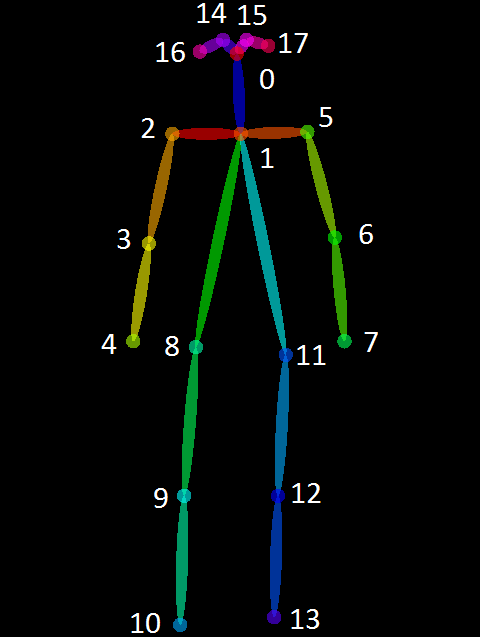
\includegraphics[scale=0.55]{./img/keypoints_openpose.png}
  \caption[Keypoints detected by OpenPose]{Keypoints detected by OpenPose \cite{cao2017realtime}}\label{fig:Keypoints detected by OpenPose}
\end{figure}

\subsection*{Convolutional Pose Machine (CPM)}
 \par Convolutional Pose Machine (CPM) use Convolutional Neural Networks (CNNs) to detect the human joint data from 2D image or video. CPMs consist of a sequence of convolutional networks that repeatedly produce 2D belief maps for the location of each part (Figure \ref{fig:eft}). At each stage, image features and belief maps produced by the previous stage are used as input \cite{Wei2016}.

\begin{figure}[htbp]
\centering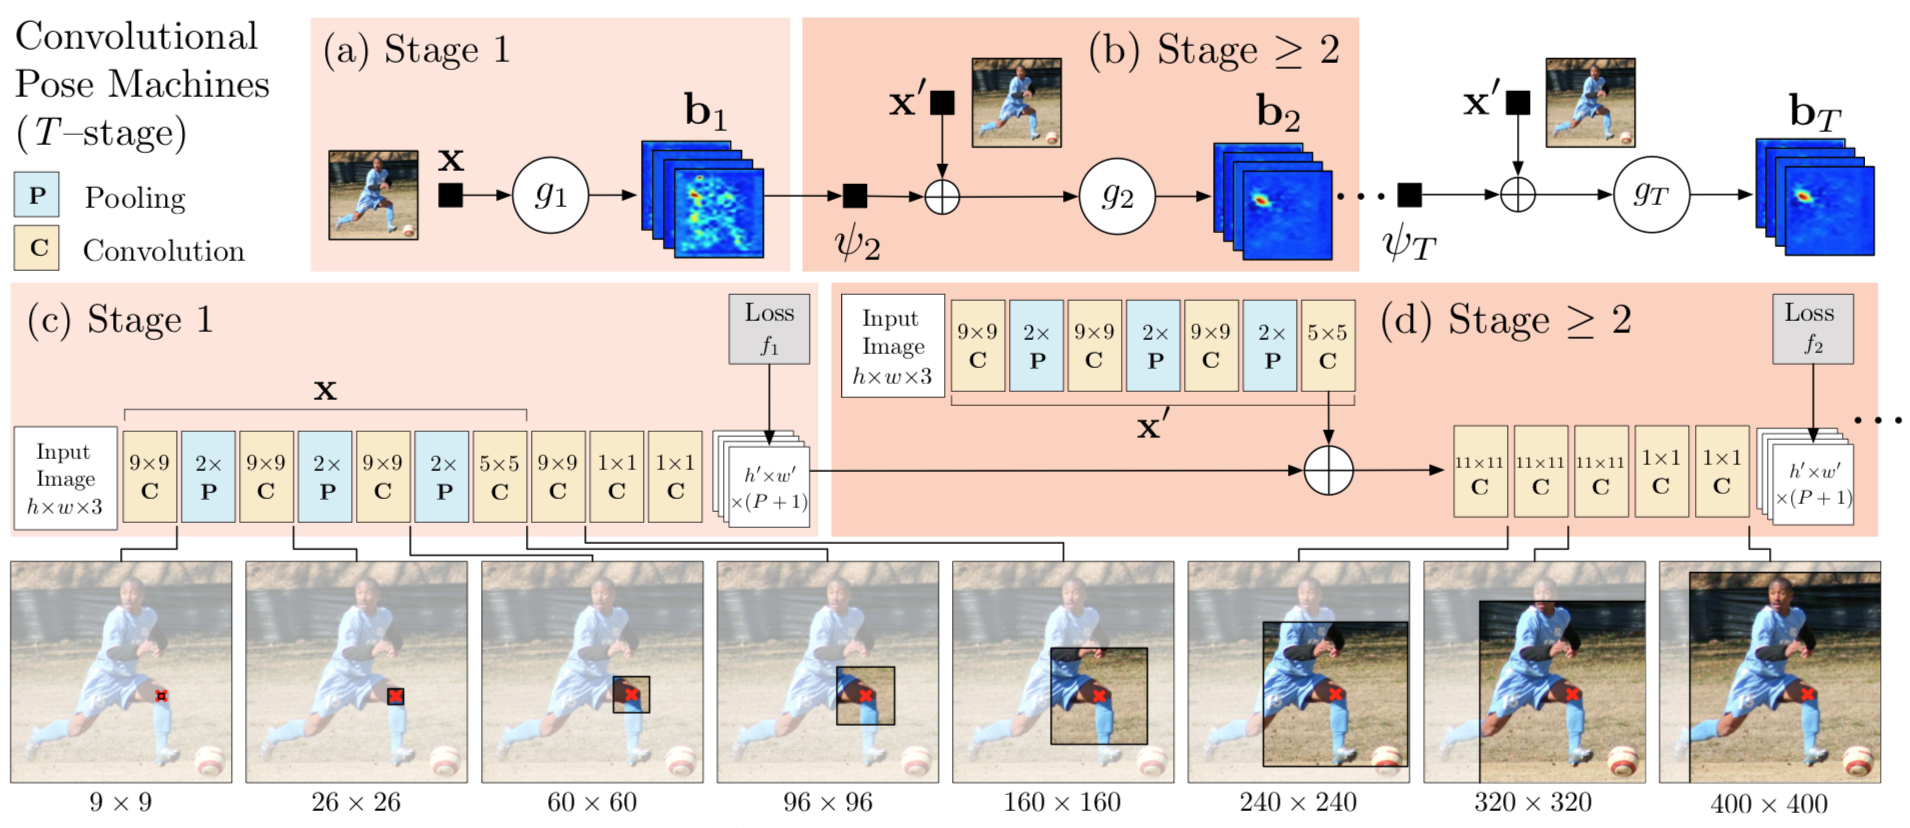
\includegraphics[width=0.9\textwidth]{./img/eft.png}
  \caption[Architecture of Convolutional Pose Machines (CPMs)]{Architecture of Convolutional Pose Machines (CPMs) \cite{Wei2016}}\label{fig:eft}
\end{figure}

\par The belief maps provide the subsequent stage an expressive non-parametric encoding of the spatial uncertainty of location for each part, allowing the CPM to learn rich image-dependent spatial models of the relationships between parts. The overall proposed multi-stage architecture is fully differentiable and therefore can be trained in an end-to-end fashion using back propagation \cite{Wei2016}.
\par At a particular stage in the CPM, the spatial context of part beliefs provides strong disambiguating cues to a subsequent stage. As a result, each stage of a CPM produces belief maps with increasingly refined estimates for the locations of each part.
\par To capture long-range interactions between parts, the design of the network in each stage of our sequential prediction framework is motivated by the goal of achieving a large receptive field on both the image and the belief maps \cite{Wei2016}.

\subsection*{OpenPose}
\par Based on CPM architecture, OpenPose is an efficient method for multi-person pose estimation what uses a non-parametric representation of association scores via Part Affinity Fields (PAFs), a set of 2D vectors field that encodes the location and orientation of limbs over the image domain.
\par The part affinity is a 2D vector field for each limb for each pixel in the area belonging to a particular limb, which encodes the direction that points from one part of the limb to the other. Each type of limb has a corresponding affinity field jointing its two associated body parts. A greedy parsing algorithm is sufficient to produce high-quality parses of body poses, which maintains efficiency even as the number of people in the image increases \cite{cao2017realtime}.
\par Figure \ref{fig:paf} illustrates the overall pipeline of OpenPose library.

\begin{figure}[htbp]
  \centering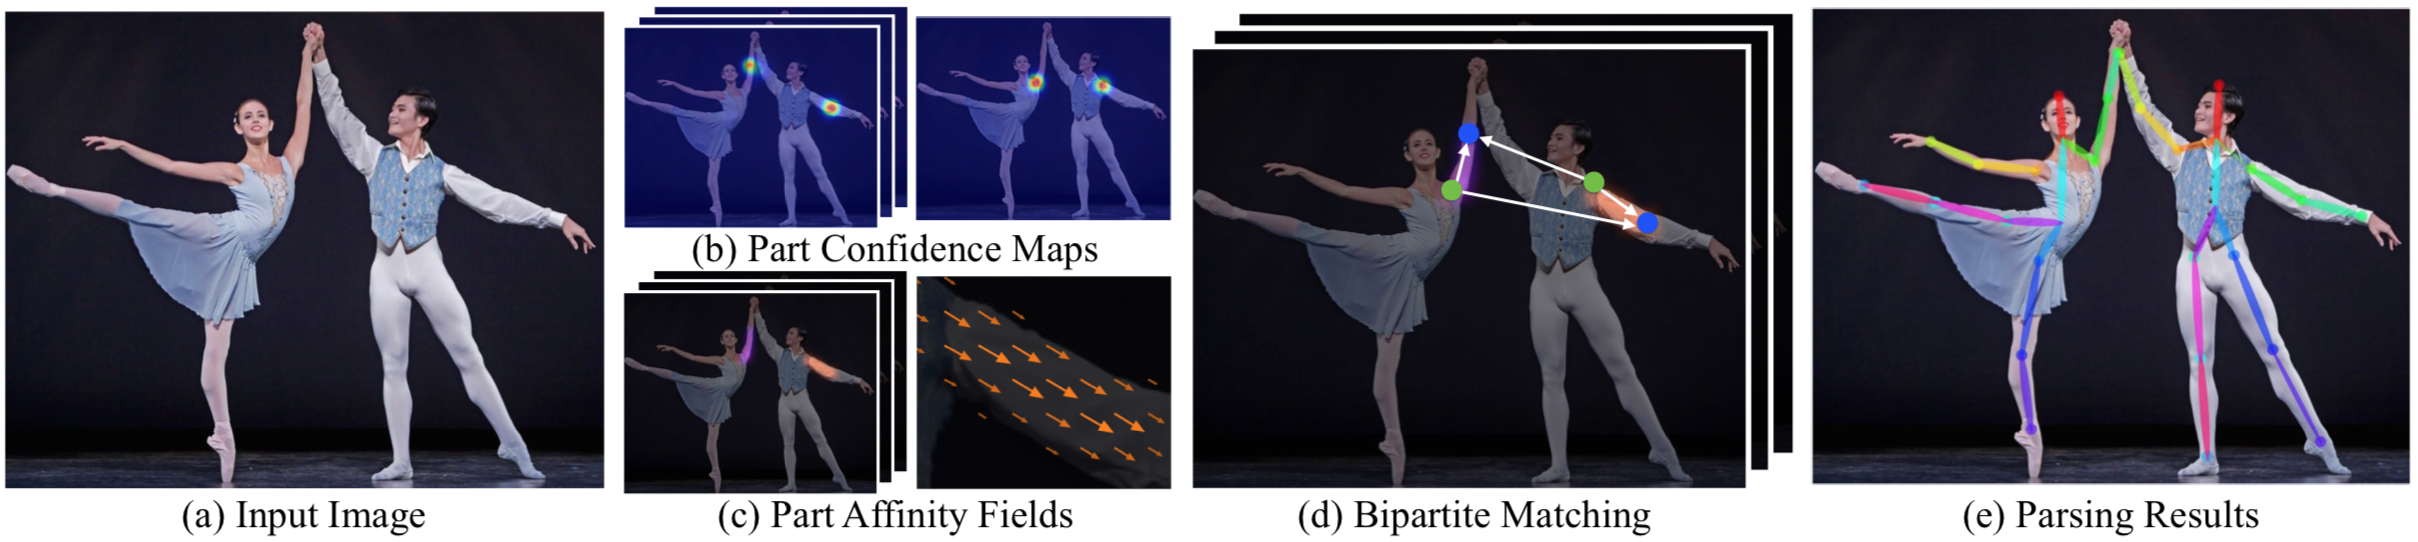
\includegraphics[width=0.8\textwidth]{./img/paf.png}
  \caption[Overall pipeline of OpenPose]{Overall pipeline of OpenPose \cite{cao2017realtime}}\label{fig:paf}
\end{figure}

\begin{itemize}
\item OpenPose takes, as input, a color image of size of $w \times h$ (Figure \ref{fig:paf}a) and produces, as output, the 2D locations of anatomical key-points for each person in the image (Figure \ref{fig:paf}e) \cite{cao2017realtime}.
\item First, a feed-forward network simultaneously predicts a set of 2D confidence maps of body part locations (Figure \ref{fig:paf}b) and a set of 2D vector fields of part affinities, which encode the degree of association between parts (Figure \ref{fig:paf}c).
\item Finally, the confidence maps and the affinity fields are parsed by greedy inference (Figure \ref{fig:paf}d) to output the 2D key points for all people in the image.
\end{itemize}

\begin{figure}[!htbp]
\centering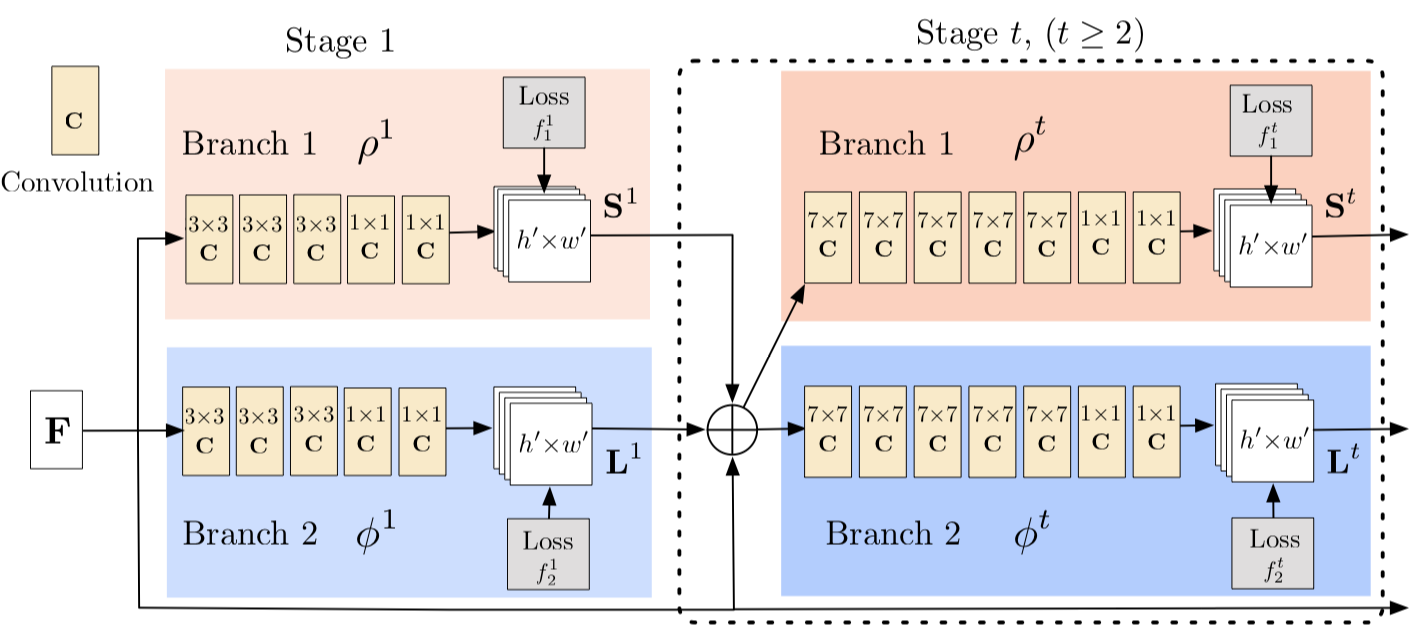
\includegraphics[width=0.9\textwidth]{./img/OpenPoseArchitecture.png}
  \caption[Architecture of the two-branch multi-stage CNN in OpenPose]{Architecture of the two-branch multi-stage CNN in OpenPose \cite{cao2017realtime}}\label{fig:architecture}
\end{figure}

\par The architecture of OpenPose, shown in Figure \ref{fig:architecture}, simultaneously predicts detection confidence maps and affinity fields that encode part-to-part association. The network is split into two branches: the top branch, shown in beige, predicts the confidence maps, and the bottom branch, shown in blue, predicts the affinity fields. Each branch is an iterative prediction architecture, Following the typical structure of a CMP, which refines the predictions over successive stages, with intermediate supervision at each stage \cite{cao2017realtime}.

\par In our proposed system, we employed OpenPose library to extract the orator's joint data from past famous 2D speech video (Figure \ref{fig:jfkexample}). We use those joint data to do template matching to get the score.
\begin{figure}[!htbp]
  \centering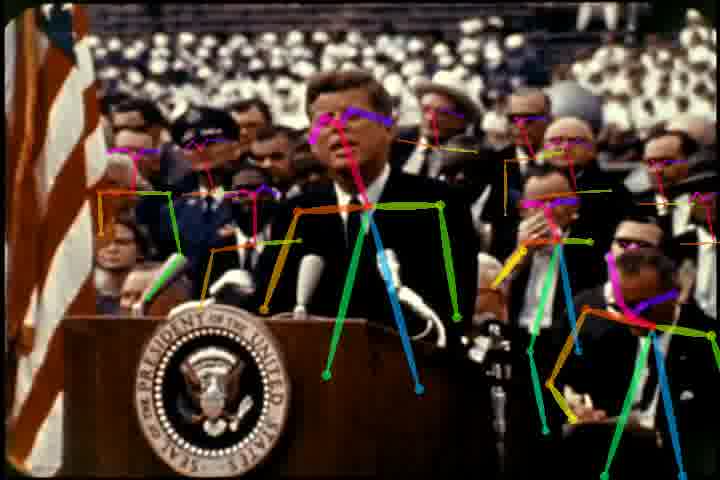
\includegraphics[width=0.9\textwidth]{./img/jfk.png}
  \caption{Joint detected by OpenPose (Example)}\label{fig:jfkexample}
\end{figure}



\section{Joint Data Extraction Method (3D)}
\par Recent advances in 3D depth cameras such as Microsoft Kinect sensors have created many opportunities for multimedia computing. The Kinect sensor lets the computer directly sense the third dimension (depth) of the players and the environment. It also understands when users talk, knows who they are when they walk up to it and can interpret their movements and translate them into a format that developers can use to build new experiences \cite{Zhang2012}.
\subsection*{Kinect V2 Sensor}
\par The Kinect V2 sensor incorporates several advanced sensing hardware. Most notably, it contains a depth sensor, a color camera, and a microphone array that provide full-body 3D motion capture, facial recognition, and voice recognition capabilities. Figure \ref{fig:kinect} shows the arrangement of the infrared (IR) camera, the color camera, and the IR illuminator. 

\begin{figure}[htbp]
  \centering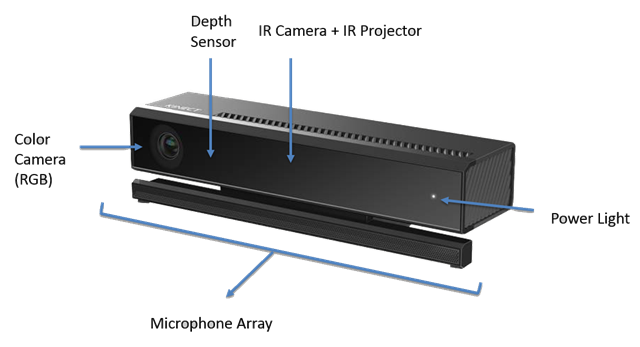
\includegraphics[width=0.7\textwidth]{./img/kinect.png}
  \caption[Microsoft Kinect V2 sensor]{Microsoft Kinect V2 sensor \cite{Fankhauser2015}}\label{fig:kinect}
\end{figure}

\par The Kinect V2 depth sensor is based on the time-of-flight measurement principle. An infrared strobe light (see Figure \ref{fig:kinect}) illuminates the scene, the light is reflected by obstacles, and the time of flight for each pixel is registered by the infrared camera. Internally, wave modulation and phase detection are used to estimate the distance to obstacles (indirect ToF)\ cite{Fankhauser2015a}. Details on the depth measurement method of the Kinect V2 are given in Sell's paper \cite{Sell}.

\subsection*{Kinect Skeletal Tracking}
\par In skeletal tracking, a human body is represented by some joints representing body parts such as head, neck, shoulders, and arms (see Figure \ref{fig:skeletonmap}). Each joint is represented by its 3D coordinates.

\begin{figure}[htbp]
  \centering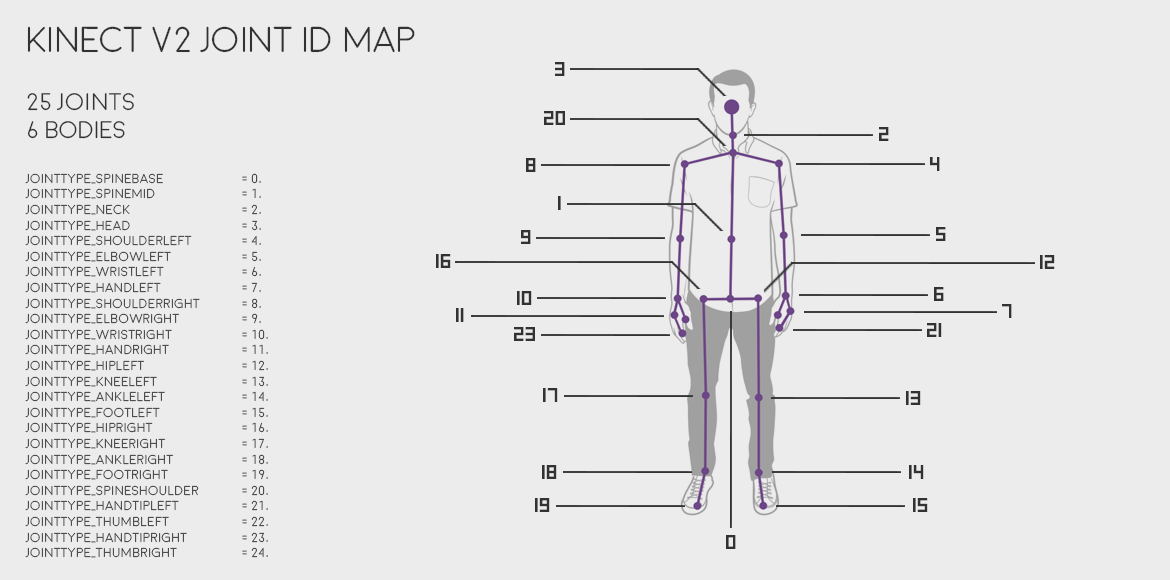
\includegraphics[width=0.8\textwidth]{./img/kinectskeleton.png}
  \caption[Microsoft Kinect V2 joint id map]{Microsoft Kinect V2 joint id map \footnotemark}\label{fig:skeletonmap}
\end{figure}

\footnotetext{https://vvvv.org/documentation/kinect}

\par Figure \ref{fig:trackingpipeline} illustrates the whole pipeline of Kinect skeletal tracking. The first step is to perform per-pixel, body-part classification. The second step is to hypothesize the body joints by finding a global centroid of probability mass through the mean shift. The final stage is to map hypothesized joints to the skeletal joints and fit a skeleton by considering both temporal continuity and prior knowledge from skeletal train data \cite{Zhang2012}.

\begin{figure}[htbp]
  \centering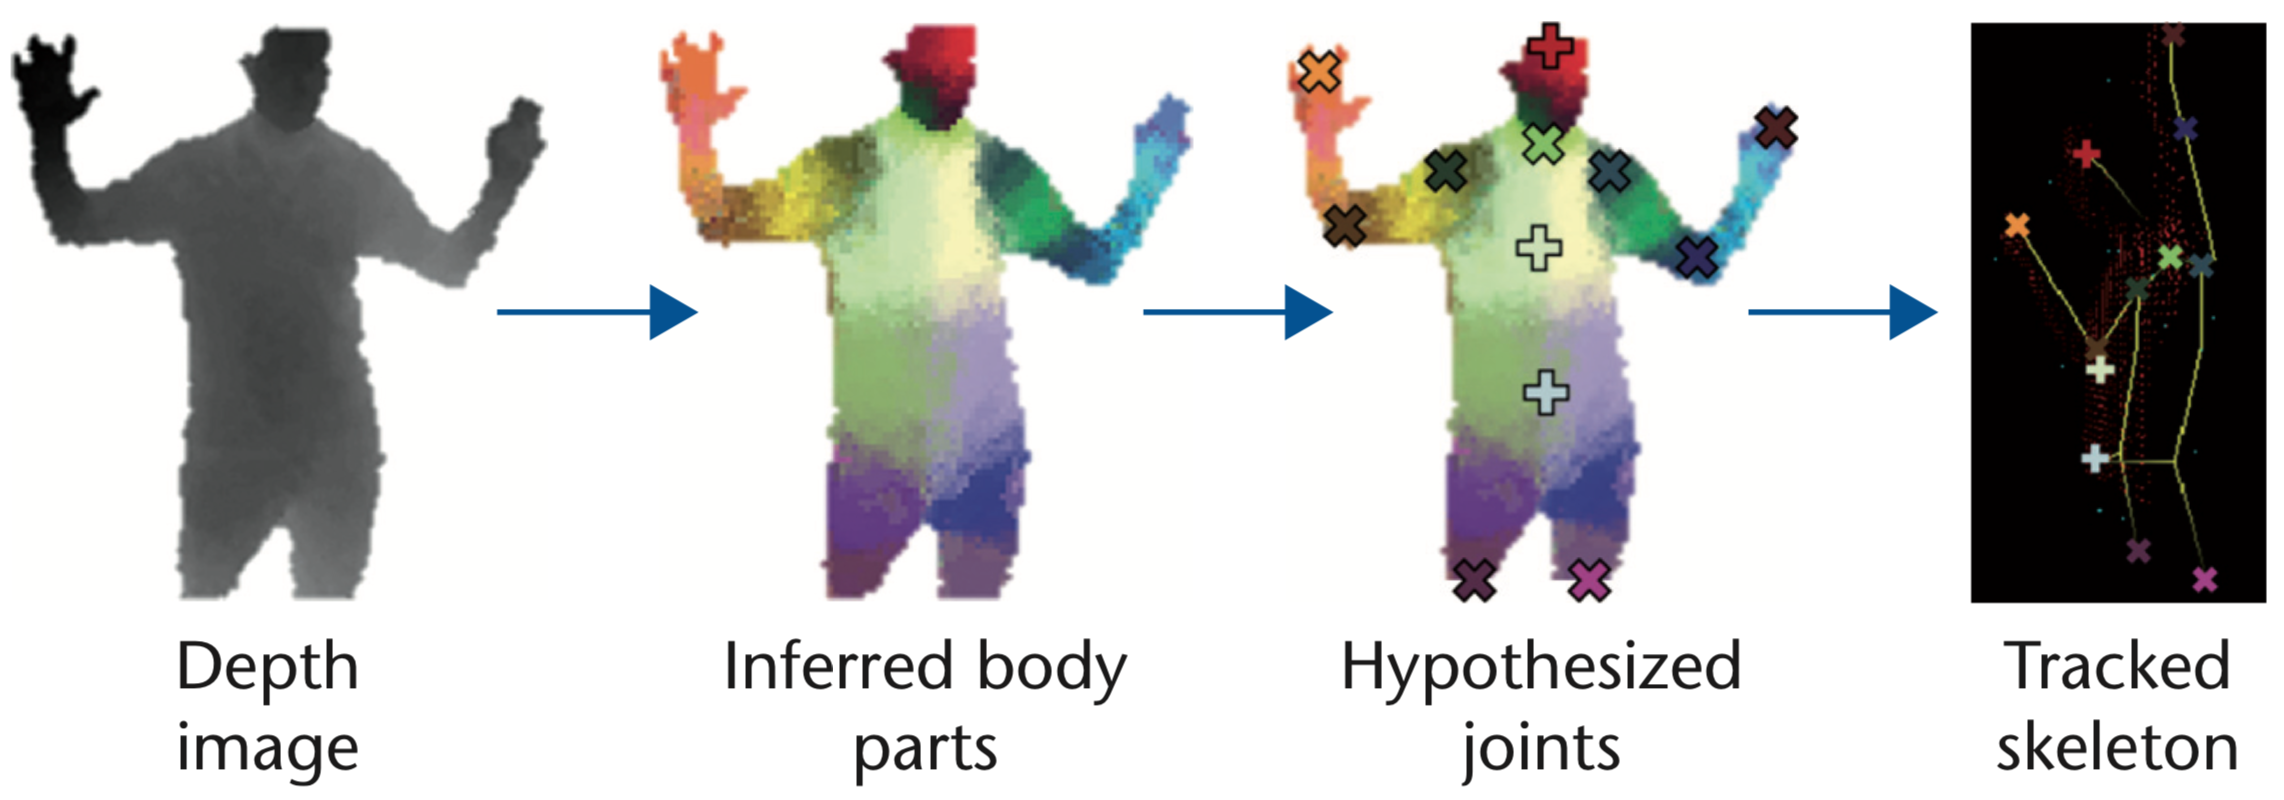
\includegraphics[width=0.65\textwidth]{./img/skeletaltracking.png}
  \caption[The Kinect skeletal tracking pipeline]{The Kinect skeletal tracking pipeline \cite{Zhang2012}}\label{fig:trackingpipeline}
\end{figure}

\par In our proposed system, we set up a Kinect V2 to extract the joint data of trainee in real-time. We only employ the 2D coordinates to fit the joint data extracted by OpenPose from the past speech.

\section{Evaluation of Presentation}

\par To evaluate the presentation skill of trainees, we need to know what kind of behaviors will have the impact on the presentation. Nguyen's research performs an observation to analysis the behaviors of presenters \cite{nguyen2015intelligent}. They collected data from a training class about public speaking skills for postgraduate students. They ask the learners to give short presentations (about one minute) in front of the audience, which includes about ten other learners and one or two coaches. The presenters can freely choose the content of the presentations. In fact, all presenters chose to talk about their research, in the ways that it can be understood by all of the audience that might come from the different fields. After each presentation, the audience gave feedbacks and suggestions on how the presentation should be improved, regarding nonverbal expressions. They set up a regular camera to record the presentations. They also set up a Microsoft Kinect to capture the whole body movement for their further signal processing, as well as behavioral studies. They stored the data from Kinect as the *.ONI files using the OpenNI SDK. They removed the unsatisfied videos (e.g. presenters moved out of the camera range) and finally collected 39 presentations of 11 presenters (four females and seven males). 
\par In their research, they use regular videos for behavioral analysis. This task was done through the collaboration with an expert in public speaking. The role of the expert was to review the recorded videos and then specifying the nonverbal cues that affected the performance of the speakers, together with the duration that they appeared. Thus, for each video, a set of behaviors was created. They collected the nonverbal cues and then annotated their appearance using the commercial software Noldus Observer XT \cite{Zimmerman2009}. Behaviors were categorized into either \textit{State event} if their duration is necessary to be studied, or \textit{Point event} otherwise. The software provided them with the statistical analysis on the appearance of these behaviors, including the number of presentations that contain the behaviors, the rate that they appeared (point events) and the percentage of time that they accounted for (Table \ref{tab:nonverbal cues}) \cite{nguyen2015intelligent}.


\begin{table}
  \caption[The list of observed nonverbal cues]{\textbf{The list of observed nonverbal cues} \cite{nguyen2015intelligent}}
\label{tab:nonverbal cues}
\resizebox{\textwidth}{!}{%
\begin{tabular}{llcclllccc}
\hline
\multirow{3}{*}{\#} & \multirow{3}{*}{Behaviors} & Event & \multirow{3}{*}{No.} & \multicolumn{3}{l}{Rate of occurrences} & \multicolumn{3}{c}{Percentage during observation} \\
 &  & Type &  & \multicolumn{3}{c}{(times/minute)} & \multicolumn{3}{c}{of the occurrences(\%)} \\ \cline{5-10} 
 &  & (S/P) &  & \multicolumn{1}{c}{M} & \multicolumn{1}{c}{SD} & \multicolumn{1}{c}{Range} & M & SD & Range \\ \hline
\multicolumn{10}{l}{\textbf{Postural behaviors}} \\
1 & (-) Shoulder too tight & S & 19 &  &  &  & 60.94 & 23.80 & 12.67 - 98.50 \\
2 & (-) Legs closed & S & 12 &  &  &  & 73.02 & 36.44 & 5.15 - 100 \\
3 & (-) Legs too stretch & S & 3 &  &  &  & 61.42 & 11.33 & 19.18 - 100 \\
4 & (-) Weight in on foot & S & 20 &  &  &  & 65.42 & 28.69 & 5.20 - 100 \\
5 & (-) Chin too high & S & 14 &  &  &  & 64.94 & 23.80 & 12.67 - 98.50 \\
6 & (-) Hands in pockets & S & 3 &  &  &  & 11.85 & 4.89 & 12.76 - 92.60 \\
7 & (+) Lean forward & S & 19 &  &  &  & 32.50 & 28.66 & 3.70 - 82.78 \\
8 & (-) Lean backward & S & 17 &  &  &  & 62.80 & 28.07 & 12.73 - 96.20 \\ \hline
\multicolumn{10}{l}{\textbf{Vocal behaviors}} \\
9 & (-) Speak too fast & S & 19 &  &  &  & 45.88 & 36.55 & 7.32 - 100 \\
10 & (-) Start too fast & P & 18 &  &  &  &  &  &  \\
11 & \begin{tabular}[c]{@{}l@{}}(-) Energy decreases \\       at the end\end{tabular} & P & 23 & 2.88 & 1.77 & 0.53 - 6.31 &  &  &  \\
12 & (+) Vocal emphasis & P & 33 & 5.51 & 4.51 & 0.59 - 17.50 &  &  &  \\
13 & (+) Suitable pause & P & 33 & 4.63 & 3.16 & 0.53 - 12.50 &  &  &  \\
14 & (-) Unsuitable pause & P & 20 & 1.73 & 1.14 & 0.53 - 5.19 &  &  &  \\
15 & (-) Monotone & S & 20 &  &  &  & 92.49 & 13.08 & 56.29 - 100 \\
16 & (-) Fillers & P & 34 & 5.17 & 4.22 & 1.44 - 19.03 &  &  &  \\
17 & (-) Stuttering & P & 12 & 1.72 & 0.83 & 0.53 - 3.42 &  &  &  \\ \hline
\multicolumn{10}{l}{\textbf{Behaviors of eye contact}} \\
18 & (-) Make eye contact & S & 39 &  &  &  & 93.81 & 8.24 & 75.00 - 100 \\
19 & (-) Contact avoidance & S & 28 &  &  &  & 9.98 & 8.47 & 1.12 - 25.00 \\
19.1 & (-) Look up to ceiling & S & 14 &  &  &  & 4.23 & 2.95 & 1.12 - 9.61 \\
19.2 & (-) Look down to floor & S & 19 &  &  &  & 7.67 & 4.67 & 2.84 - 14.17 \\
19.3 & (-) Look at hands & S & 11 &  &  &  & 10.24 & 3.15 & 4.40 - 13.15 \\ \hline
\multicolumn{10}{l}{\textbf{Behaviors related to facial expression}} \\
20 & (+) Facial mimicry & S & 30 &  &  &  & 39.31 & 25.97 & 4.50 - 91.81 \\
21 & (-) Smile & S & 22 &  &  &  & 13.62 & 11.54 & 3.54 - 41.08 \\
22 & (-) Flat face & S & 8 &  &  &  & 80.61 & 24.16 & 40.41 - 100 \\ \hline
\multicolumn{10}{l}{\textbf{Behaviors related to whole body movement}} \\
23 & (-) Too much movement & S & 11 &  &  &  & 42.21 & 25.97 & 4.50 - 91.81 \\
24 & (-) Too little movement & S & 23 &  &  &  & 50.62 & 29.21 & 10.05 - 100 \\
25 & (-) Step backward & P & 31 & 1.83 & 1.27 & 0.36 - 4.36 &  &  &  \\
26 & (+) Step forward & P & 34 & 2.06 & 1.04 & 0.59 - 4.61 &  &  &  \\ \hline
\multicolumn{10}{l}{\textbf{Behaviors related to hand gesture}} \\
\multicolumn{10}{l}{\textit{Amount of hand gesture}} \\
27 & Hand gesture occur & P & 38 & 16.83 & 7.15 & 0.93 - 28.42 &  &  &  \\
28 & (-) Too little gestures & S & 20 &  &  &  & 69.55 & 34.64 & 17.21 - 100 \\
29 & (-) Too much gestures & S & 10 &  &  &  & 61.49 & 31.82 & 27.34 - 96.10 \\ \hline
\multicolumn{10}{l}{Quality of hand gestures} \\
30 & (-) Bounded gestures & P & 30 & 6.75 & 5.33 & 1.00 - 19.77 &  &  &  \\
31 & (+) Relaxed gestures & P & 29 & 7.41 & 4.95 & 1.15 - 15.79 &  &  &  \\
32 & (-) Casual gestures & P & 10 & 5.16 & 3.14 & 1.56 - 10.28 &  &  &  \\
33 & (-) Uncompleted gesture & P & 27 & 3.23 & 2.78 & 0.93 - 10.27 &  &  &  \\
34 & (+) Gestural emphasis & P & 20 & 4.43 & 4.05 & 0.36 - 11.99 &  &  &  \\
35 & (-) Repeated gestures & P & 31 & 6.57 & 2.49 & 1.09 - 12.31 &  &  &  \\ \hline
\end{tabular}%
}
\end{table}
\newpage
\par The observed behaviors can be separated based on the nonverbal channels that they were generated: (1) Posture (the static configuration of body), (2) Voice (concerning the paralinguistic characteristics), (3) Eye contact, (4) Facial Expression, (5) Globe body movement, (6) Hand gesture. This method of categorization is similar to the literature of public speaking skills \cite{rodman1996style}. From Nguyen's observation, as well as advices from the expert, they find the following aspects are the most important:

\begin{itemize}
  \item \textit{Eye Contact} : Similar to social interaction, maintaining good eye contact is the first thing the presenters must keep in mind. It initiates and strengthens the connection between them and the audience (\#18, 19 in Table \ref{tab:nonverbal cues}). It might have the first and foremost influence on the performance of a presentation, as well as regular communications \cite{Zimmerman2009}.
  \item \textit{Amount of energy} : This aspect concerns the dynamic characteristics of a presentation, thus can reflect the internal state of the presenters. It has the impact on most behaviors that they have found (except posture as the static channel). For example, the amount of whole body movement (\#23, 24), the amount of hand gesture (\#28, 29), vocal behaviors (partly via tempo, emphases) and most features of hand gesture.
  \item \textit{Variety} : The presentations with strong variations significantly increase the attention of the audience \cite{nguyen2015intelligent}. Lacking variation results in monotone (\#15), flat face (\#22), and hand gesture repeated (\#35). In fact, variety can be separated as one single measurement to analyze a presentation. It takes the role as rhythm in music. Even a beautiful piece of music, without changes in rhythm, will steadily lose the attention of the audience.  

\end{itemize}

\par To evaluate the effectiveness of our proposed system, we need to select some import cues from Nguyen's research. We made a previous experiment, in which we let the evaluator score the trainee's presentation with all 35 cues. However, We find it's too hard for the evaluator to score by all those cues. So we select 20 most occurred cues, and we make a evaluate sheet, like table \ref{tab:evalutioncues} to evaluate the presentation skills of the trainees before and after the training. We will explain the details about our experiment in chapter 5.

\begin{table}[]
\centering
\caption{Nonverbal cues for evaluation}
\label{tab:evalutioncues}
\begin{tabular}{clc}
\hline
\multirow{3}{*}{\textbf{\#}} & \multicolumn{1}{c}{\multirow{3}{*}{Behaviors}} & \multirow{2}{*}{Event Type} \\
 & \multicolumn{1}{c}{} &  \\
 & \multicolumn{1}{c}{} & (S/P) \\ \hline
\multicolumn{2}{l}{Postural behaviors} &  \\
1 & (-) Hands in pockets & S \\
2 & (+) Lean forward & S \\
3 & (-) Lean backward & S \\ \hline
\multicolumn{2}{l}{Vocal behaviors} &  \\
4 & (-) Speak too fast & S \\
5 & (+) Vocal emphasis & P \\
6 & (+) Suitable pause & P \\
7 & (-) Unsuitable pause & P \\ \hline
\multicolumn{2}{l}{Behaviors of eye contact} &  \\
8 & (-) Make eye contact & S \\
9 & (-) Contact avoidance & S \\
10 & (-) Look up to ceiling & S \\
11 & (-) Look down to floor & S \\ \hline
\multicolumn{2}{l}{Behaviors related to facial expression} &  \\
12 & (-) Smile & S \\
13 & (-) Flat face & S \\ \hline
\multicolumn{2}{l}{Behaviors related to whole body movement} &  \\
14 & (-) Too much movement & S \\
15 & (-) Too little movement & S \\
16 & (-) Step backward & P \\
17 & (+) Step forward & P \\ \hline
\multicolumn{3}{l}{Behaviors related to hand gesture} \\
18 & (+) Hand gesture occur & P \\
19 & (-) Too little gestures & S \\
20 & (-) Too much gestures & S \\ \hline
\end{tabular}
\end{table}

